\section{System Identification Setup}%
\label{sec:sys_iden}
In this thesis understanding how objects behave as a result of input sent to the robot is captured by \textit{system models}. System identification aims to create a system model that best relates an input sequence to an output sequence. Three types of system models are categorized, data-driven-, hybrid- and analytic system models. Data-driven models are generated by only using \ac{IO} data, and hybrid system models provide a predetermined structure between the input and output with several variables to be determined by \ac{IO} data, such as the object's dimensions or weight. Analytic models are fully defined and thus do not use any \ac{IO} data. Note, this section eleborates on how to collect an \ac{IO} data set, and does not eleborate on system identification methods themselves. System identification methods are relocated to the future work section.\bs

An example of a system model is the drive model for the robot. The model estimates the robot's trajectory when input is sent to the robot. For a specified range of inputs that can be sent to the robot, a system model can predict the possible future states that a robot can reach for a small number of time steps. Using this method, a prediction can be made that estimates if states are reachable from the current state and which states cannot be reached.\bs

To generate a data-driven- or hybrid system model, \ac{IO} data is required that is collected by sending input to the robot and recording the output response. Now a method for data collection is presented to collect data for drive and push applications.\bs

The \ac{IO} data set is defined as:
\[ \ac{IO} \textrm{ data set} = \left[(u_1(k), y_1(k)), \dots, (u_g(k), y_g(k)) \right]\]
\[= \left[(u_1(1), \cdots u_1(a), y_1(1), \cdots y_1(a)), \dots (u_g(1), \cdots u_g(a), y_g(1), \cdots, y_g(b)) \right]\]
Where $k$ is the time step, $(u_\mathit{id}, y_\mathit{id})$ is a \ac{IO} sequence with identifier \textit{id}, $m$ is the number of sequences in the \ac{IO} data set, $a$ is the number of inputs and outputs in sequence with identifier $1$, $b$ is the number of inputs and outputs in sequence with identifier $g$. With $g, a, b \in \gls{Rnonnegative}$\bs

\begin{figure}[H]
    \centering
    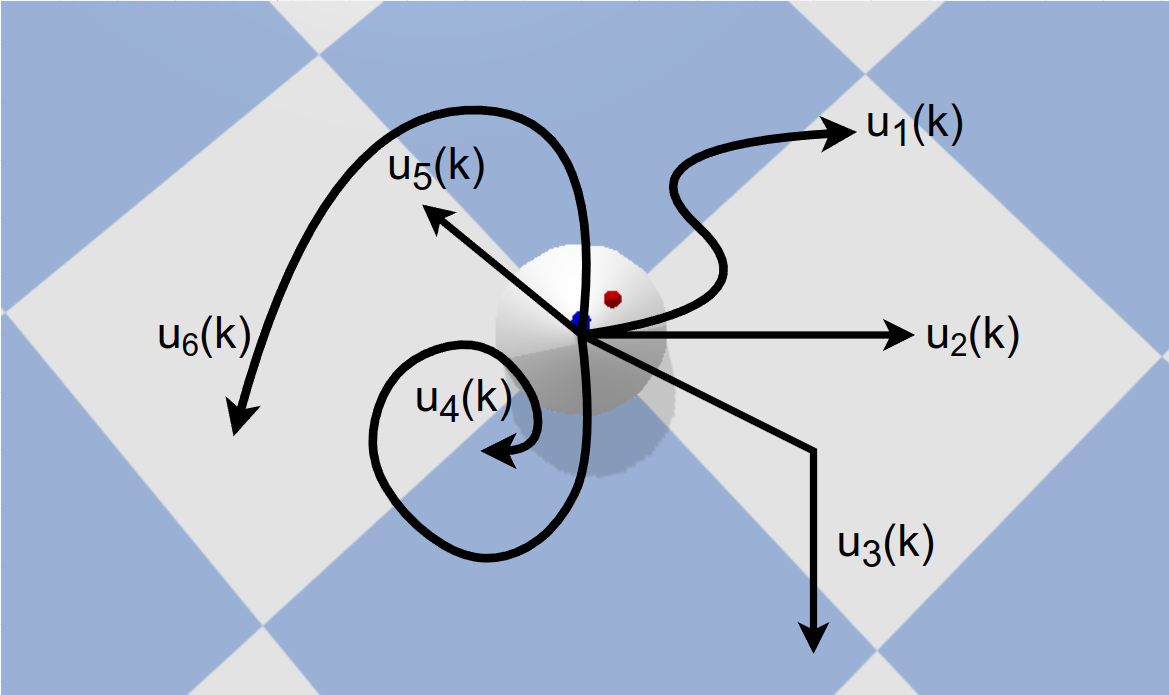
\includegraphics[width=0.7\textwidth]{figures/required_background/collect_io_robot}
    \caption{A top view of the point robot with five input sequences. The input sequences are executed\\on the robot and the output responses are recorded, together the in- and output sequences form a \ac{IO} data set.}%
    \label{fig:collect_io_robot}
\end{figure}

The initial pose does not affect a driving model's collection of an \ac{IO} sequence. At the very least, the robot should not collide with other objects during data collection. Opposite to collecting \ac{IO} data for a driving model, sending input to generate a \ac{IO} sequence for the robot-pushing model requires a predefined initial pose. That pose is relative to the object to push, as visualized in the following figure.\bs

\begin{figure}[H]\ContinuedFloat
    \centering
    \begin{subfigure}{\textwidth}
    \centering
    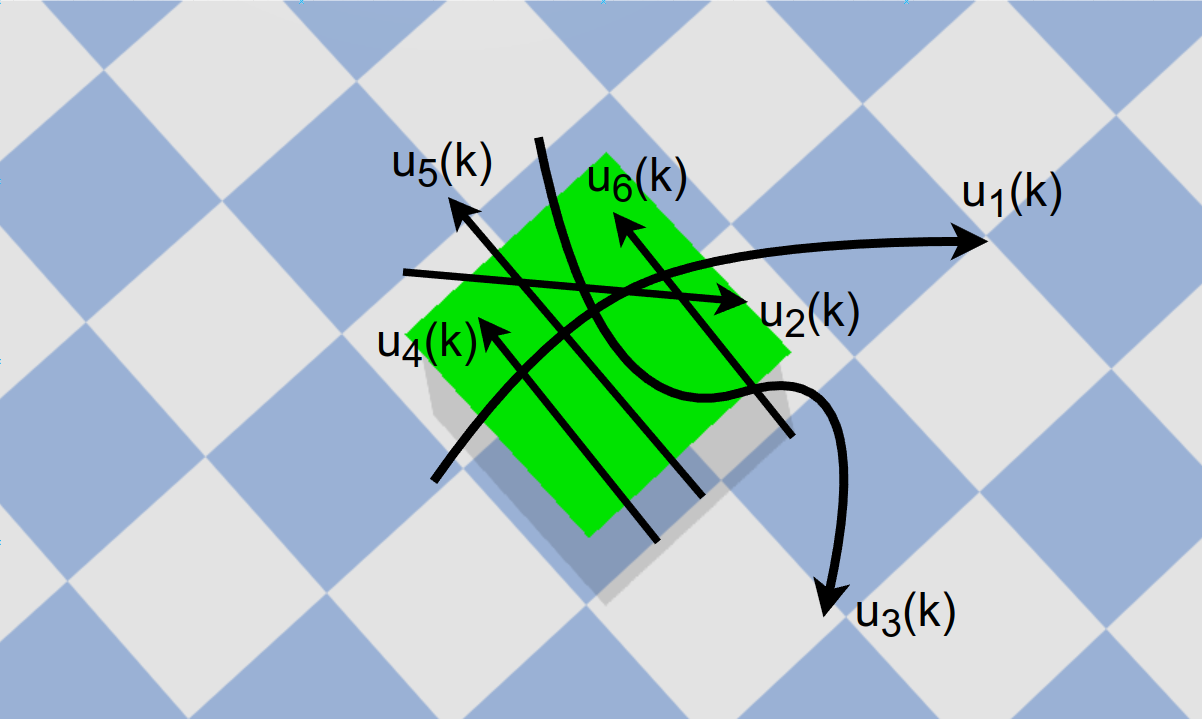
\includegraphics[width=0.7\textwidth]{figures/required_background/collect_io_data_object}
    \caption{A top view of a box object with six input sequences.}%
    \label{subfig:collect_io_object_arrows}
    \end{subfigure}

    \begin{subfigure}{\textwidth}
    \centering
    
\includegraphics[width=0.7\textwidth]{figures/required_background/collect_io_data_obj_and_robot}
    \caption{The robot driving to toward the initial pose to then apply input sequence $u_1(k)$ and collect output sequence $y_1(k)$.}%
    \label{subfig:collect_io_object_goto_init}
    \end{subfigure}
    \caption{The roobt collecting an \ac{IO} data sequence by first driving toward the initial pose at the start of an arrow. Then the corresponding input is sent toward the robot, and the robot and the object's output response is collected to form a \ac{IO} sequence. The \ac{IO} data set then consists of all six \ac{IO} data sequences.}%
    \label{fig:collect_io_object}
\end{figure}

A top view of the point robot with five input sequences. The input sequences are executed\\on the robot and the output responses are recorded, together the in- and output sequences form a \ac{IO} data set.

The quality of a system model resides in the dynamics it can capture from the system. In order to create models that capture a large portion of the dynamics, system identification methods need an \ac{IO} data set that captures these dynamics. It must be recorded when the system is persistently exited to create \ac{IO} sequences that capture the dynamics. Creating input that persistently excites the system is out of the scope of this thesis.\bs

Only a method for data collection is preset, which is fully integrated with the proposed framework. System identification is not implemented or tested; instead, analytic models are used for two time-related reasons. Firstly creating the implementation module itself takes too much time. Secondly, collecting enough \ac{IO} data to generate a system model is time wise very costly. Thus, time is saved by using several analytic system models instead of implementing a system identification module. The replacement moves to focus from \quotes{which system identification method yields a system model that most accurately describes a dynamic model?} to \quotes{which system model in the set of available models most accurately describes a dynamic model?}. The analytic system models are not opting for modelling the drive or push model as accurately as they possibly can, thus severe model mismatch should be expected.\bs

Related to system identification is \textit{system classification}, a symbolic model that indicates the accordance of objects. In this thesis objects are initially classified as UNKNOWN, a test determines if objects are movable or unmovable and classify them as MOVABLE or UNMOVABLE, indicating that they can or cannot be pushed. That test is presented in \Cref{sec:halgorithm}.\bs
